%! Author = hilfiker
%! Date = 21.07.2022

% Preamble
\documentclass[11pt]{article}

% Packages
\usepackage{amsmath} % Formulas in document
\usepackage{pdflscape} % Landscaped pages in Pdf
\usepackage[a4paper, margin=0.8in]{geometry} % Set the margin and size of a page
\usepackage[hidelinks]{hyperref} % Remove Boxes around Hyperlinks
\usepackage{lastpage} % Custom page numbering
\usepackage{pgfgantt} % Gantt-Tables
\usepackage{fancyhdr}
\usepackage{graphicx}
\usepackage{xspace}
\usepackage{mwe}
\usepackage{caption}
\usepackage{tcolorbox} % Custom page numbering

\usepackage{titling}
\usepackage{textcomp}
\usepackage{wasysym}
\usepackage[utf8]{inputenc}
\usepackage[T1]{fontenc}
\usepackage{enumerate}
\renewcommand\maketitlehooka{\null\mbox{}\vfill}
\renewcommand\maketitlehookd{\vfill\null}

\renewcommand*\contentsname{Inhaltsverzeichnis}
\renewcommand{\figurename}{Abb.}

% Configure page numbering & footer
\pagestyle{fancy}
\fancyhf{}
\lfoot{Tobias Hilfiker}
\cfoot{Seite \thepage \hspace{1pt} von \pageref{LastPage}}
\rfoot{\today}

% Methadata
\title{
    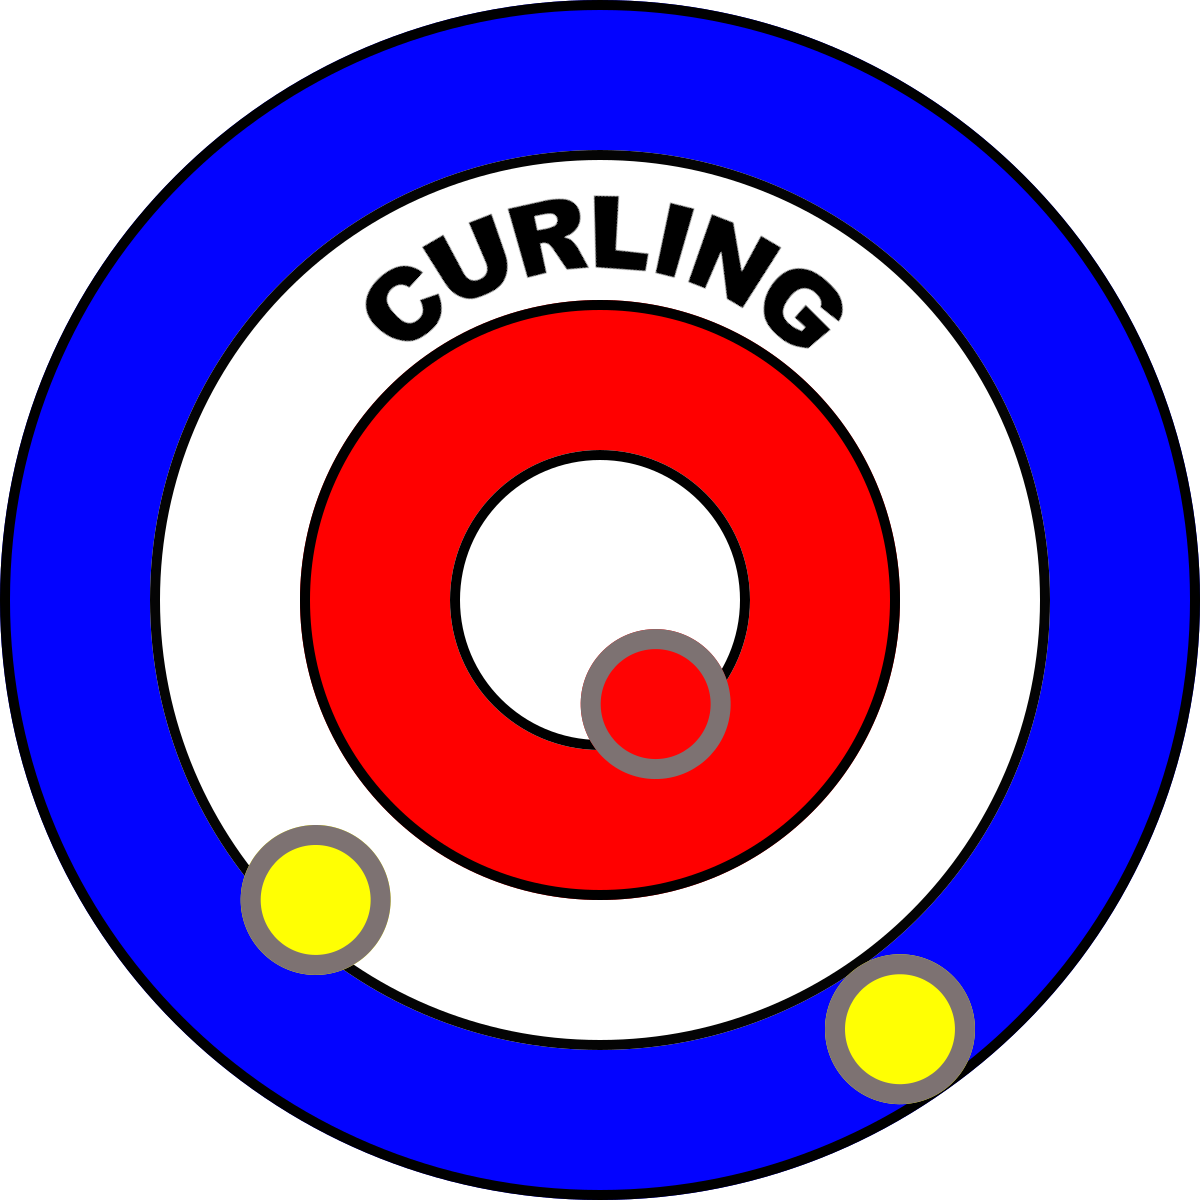
\includegraphics[width=\textwidth]{media/curling_logo}
    \begin{center}
        Modul 152 \\
        Multimediainhalte in einen Webauftritt integrieren\\
        E-Portfolio
    \end{center}}
\author{Tobias Hilfiker}
\date{\today}

% Document
\begin{document}

    %Kapitel Frontpage
    \begin{titlingpage}
        \maketitle
    \end{titlingpage}
    \pagebreak

    %Kapitel Table of contents
    \tableofcontents
    \pagebreak

    %Kapitel 1 - Einleitung
    \section{Einleitung}
    Im vorgehenden Storyboard habe ich die Umsetzung der Webseite beschrieben, welche ich im Rahmen dieses Projektes umsetzen darf. Während des
    E-Portfolios sollten folgende Unteraufgaben erfüllt werden:

    \begin{itemize}
        \item Responsive-Webseite anhand des Mockups im Storyboard umsetzen
        \item Video über das gewählte Thema filmen und schneiden
        \item Minimum drei Bilder machen und diese mit einer Bildmanipulation versehen
        \item Multimediaelemente aus den letzten zwei Punkten in die Webseite einbinden
        \item Prozess der oben genannten Punkten in dieser Dokumentation dokumentieren
    \end{itemize}
    \pagebreak

    %Kapitel 2 - Webseite
    \section{Webseite}

    %Kapitel 2.1 - Eingesetzte Technologien
    \subsection{Eingesetzte Technologien}

    %Kapitel 2.2 - Reflexion Webseite
    \subsection{Reflexion Webseite}

    %Kapitel 3 - Video
    \section{Video}
    In den folgenden Kapiteln werde ich erklären, wie ich das Video gefilmt habe und was die Schwierigkeiten dabei waren. Zudem werde ich
    erläutern, wie ich das Video geschnitten habe und über den ganzen Prozess reflektieren.

    %Kapitel 3.1 - Erstellung Video
    \subsection{Filmen Video}
    Mich stellte die von mir gesetzte Anforderung, dass ich gefilmt haben wollte, wie verschiedene Steine gespielt werden, vor eine Challenge.
    Denn am besten sieht es aus, wenn man Steine während dem Spiel von oben filmt. Wenn dies zum Beispiel an einer WM oder Olympia gemacht wird,
    werden über dem Spielfeld sogenannte Seilkameras aufgehängt. Diese sind an Seilen aufgehängt und hängen über dem Spielfeld. Mittels Motoren
    und Zugseilen können diese dann ferngesteuert werden und über das Spielfeld flitzen. Allerdings haben wir in der Curlinghalle in St. Gallen
    keine solchen Einrichtungen. Daher muss ich mir anders behelfen.\\
    Für mich war es am einfachsten, eine Drohne zu verwenden. Auch das war aber nicht sehr einfach. Denn in der Halle selbst habe ich aufgrund
    des Metalldachs keinen GPS-Empfang, was dazu führt, dass die Drohne nicht stabil an Ort und Stelle bleibt.
    Als Drohne habe ich eine DJI Mavic Air verwendet, welche eigentlich auch über ein sogenanntes \"FocusTrack\" Feature verfügt. Dieses erlaubt dem
    Pilot der Drohne, Objekte auszuwählen, welcher die Drohne automatisch folgt. Dieses habe ich aus folgenden zwei Gründen nicht verwendet
    / verwenden können:

    \begin{enumerate}
        \item Aufgrund des fehlenden GPS erlaubte mir die Drohne gar nicht, FocusTrack zu verwenden
        \item Es war mir zu riskant, die Drohne in der Halle automatisch fliegen zu lassen. Die Drohne durfte nämlich auf keinen Fall abstürzen,
        da sonst das Eis beschädigt werden könnte. Einfach unkontrolliert aufsteigen sollte sie aber auch nicht, da nach wenigen Metern
        die Hallendecke kommt.
    \end{enumerate}
    Daher blieb mir nichts anderes übrig, als die Drohne manuell hinter dem gespielten Stein hinterherzufliegen. Da dies recht anspruchsvoll ist
    und ich nicht gerade für mein Flugkönnen bekannt bin, habe ich einen Kollegen, welcher auch einige Jahre Curling gespielt hat, angefragt, ob er
    mir hilft zu filmen. Er fliegt in der Freizeit FPV-Drohnen (Drohne mit VR-Brille, mit welcher man die Perspektive der Drohne sieht) und kennt
    sich daher sehr gut mit dem Fliegen der Drohnen aus.\\
    Ich habe zudem geschaut, dass nicht zu viele Personen in der Halle sind, damit einerseits nicht zu viele zusätzliche Personen auf den Bildern
    sind, andererseits dass wir mit unseren Drohnenflügen nicht viele Personen in Gefahr bringen / stören.\\
    Abgesehen von den Anfangsschwierigkeiten mit dem GPS hatten wir während des Filmens keine Probleme.

    %Kapitel 3.2 - Schnitt des Videos
    \subsection{Schnitt des Videos}
    Ich war mir lange nicht sicher, wie ich das Video schneiden soll. Da ich mehrere einzelne Clips hatte, die ich einerseits kürzen und dann
    aneinanderreihen musste, brauchte ich ein Tool, welches dafür gut genug war. Bisher hatte ich Videos immer auf dem Handy geschnitten, was
    besonders mit den grossen Videodateien, welche die Drohne gespeichert hatte, sehr mühsam ist. Zudem hatte ich etwas Erfahrung mit Windows
    Movie Maker, allerdings gibt es diesen bereits seit Windows 8 nicht mehr. Da ich über die Schule ein Abonnement für die Adobe Creative Cloud
    habe, habe ich mich dann entschieden, ein Tool daraus zu nutzen. Da ich bereits mit Adobe Premiere Pro gearbeitet hatte und wusste, dass
    es sehr umfänglich und umständlich ist, wollte ich dieses Mal Adobe Premiere Rush ausprobieren.\\
    Premiere Rush ist sehr simpel ausgelegt, bietet mir aber alle Tools, die ich benötige. Zudem sind die Output-Files in einer sehr hohen
    Qualität, womit ich vor allem bei Movie Maker in der Vergangenheit Probleme hatte.\\
    Da Premiere Rush so einfach ausgelegt ist, war es auch keine grosse Sache das Video zu schneiden. Manchmal hatte der Laptop etwas Mühe,
    das Video immer flüssig abzuspielen. Ich kann aber nicht definitiv sagen, ob die CPU oder der RAM zu wenig Leistung hatte und so das Programm
    etwas blockiert hat.\\
    Ansonsten hat mich das Programm überzeugt, sprich ich werde es auch ein anderes Mal wieder verwenden, wenn ich ein Video schneiden muss.

    %Kapitel 3.3 - Reflexion Video
    \subsection{Reflexion Video}

    %Kapitel 4 - Bildmanipulationen
    \section{Bildmanipulationen}

    %Kapitel 4.1 - Bildmanipulation 1
    \subsection{Bildmanipulation 1}

    %Kapitel 4.2 - Bildmanipulation 2
    \subsection{Bildmanipulation 2}

    %Kapitel 4.3 - Bildmanipulation 3
    \subsection{Bildmanipulation 3}

    %Kapitel 4.4 - Reflexion Bildmanipulationen
    \subsection{Reflexion Bildmanipulationen}

    %Kapitel 5 - Fazit
    \section{Fazit}

\end{document}